\documentclass[12pt,a4paper]{article}

\usepackage{inputenc}
\usepackage[russian]{babel}
% \usepackage{hyperref}
\usepackage{indentfirst}
\usepackage{amsmath}
\usepackage{graphicx}
\usepackage{tikz}
\usepackage{listings}
\usepackage{xcolor}
\usepackage[width=17cm,top=2cm,height=26cm]{geometry}

\definecolor{dkgreen}{rgb}{0,0.6,0}
\definecolor{gray}{rgb}{0.5,0.5,0.5}
\definecolor{mauve}{rgb}{0.58,0,0.82}

\lstset{
	%frame=tb,
	language=C++,
	extendedchars=\true%\color{mauve},
	aboveskip=3mm,
	belowskip=3mm,
	showstringspaces=false,
	columns=flexible,
	basicstyle={\small\ttfamily},
	numbers=none,
	numberstyle=\tiny\color{gray},
	keywordstyle=\color{blue},
	commentstyle=\color{dkgreen},
	stringstyle=\color{mauve},
	breaklines=true,
	breakatwhitespace=true,
	tabsize=3
}

\begin{document}
	
	\thispagestyle{empty}
	
	\begin{figure}
		\centering
		
\includegraphics[width=80pt]{figures/spbu_grey.png}
	\end{figure}
	
	\begin{center}
		Федеральное государственное бюджетное \\образовательное учреждение высшего образования \\<<Санкт-Петербургский государственный университет>>
		
		(СПбГУ)
	\end{center}
	
	\vspace{1em}
	УДК 52-17, 519.63, 51-71, 537.876.2
	
	\vspace{5em}
	\begin{center}
		ОТЧЕТ
		
		О ЛАБОРАТОРНОЙ РАБОТЕ
		
		\vspace{2em}
		по дисциплине <<Вычислительный практикум>> \\ по теме
		
		РАЗНОСТНЫЕ МЕТОДЫ РЕШЕНИЯ УРАВНЕНИЯ ПЕРЕНОСА. СХЕМА ЛАКСА
	\end{center}
	
	\vspace{14em}
	\begin{flushleft}
		Руководитель ЛР,\\
		старший научный сотрудник\\
		кафедры астрофизики,\\
		доцент,\\
		к.ф.-м.н. С.~А. Хайбрахманов
	\end{flushleft}
	
	\vspace{1em}
	\begin{flushright}
		Исполнители:\\
		студентка 4 курса В.~А. Кобозева,\\
		студентка 4 курса А.~Д. Лунченко
	\end{flushright}
	
	\vspace{3em}
	\begin{center}
		\textcolor{gray}{Санкт-Петербург}\\ \textcolor{gray}{2023}
	\end{center}
	
	\tableofcontents\newpage
	
	\section{Введение}
	Данная работа посвящена аналитическому и численному исследованию консервативного метода Лакса для численного решения одномерного уравнения переноса. Основной задачей является изучение разностных методов решения уравнения переноса на примере схемы Лакса. Дополнительно в работе предлагается провести численное исследование системы линейных уравнений гиперболического типа, полученных из системы уравнений Максвелла, и оценить точность полученных результатов. Результаты работы будут представлены в~виде программы для ЭВМ, которая позволит решать указанные задачи с использованием консервативного метода Лакса. Главная цель работы: изучить разностные методы решения уравнения переноса на примере схемы Лакса.
	
	В следующем разделе мы поговорим о постановке задачи, а также укажем условие дополнительной задачи. В третьем разделе будет рассказано о методе расчета, а также об~исследовании свойств схемы, таких как устойчивость, дифуузия и дисперсия и порядок аппроксимации, в конце раздела будет показан алгоритм решения поставленной задачи. Раздел 4 повествует о деталях программной реализации. В разделе 5 мы приводим результаты исследования, дополняя их графиками. Шестой раздел посвящен решению дополнительной задачи. В последнем разделе мы рассуждаем об общих выводах по всей работе.
	
	\section{Постановка задачи}
	Многие математические модели физических процессов приводят к дифференциальным уравнениям в частных производных. Обычно в качестве независимых переменных выбирают время $t$ и координату $\vec{r} = \{x, y, z\}$ (в декартовой системе координат).
	
	В данной работе рассматривается одномерное уравнение переноса
	\begin{equation}
		\frac{\partial u(x,t)}{\partial t} + a\,\frac{\partial u(x,t)}{\partial x} = 0,
	\end{equation}
	где $a = 1$ --- скорость переноса профиля.\\
	Начальные условия:
	\begin{equation}
		u(x, 0) = 
		\begin{cases}
			0.4, & x < 0.4,\\
			0.8, & 0.4 \leq x \leq 0.6,\\
			0.4, & x > 0.6.
		\end{cases}
	\end{equation}
	Граничные условия --- периодические, то есть функция имеет некоторый период $L$, равный длине отрезка $[x_L; x_R] \ni x$ в области поиска решений $G(x, t) = \{(x, t) \,|\, x \in [0; 1], t \geq 0\}$.
	
	\subsection{Дополнительная задача}
	Дана система уравнений Максвелла
	\begin{align}
		&\nabla \cdot \mathbf{D} = 4\pi\rho,\label{Maxwell1}\\
		&\nabla \cdot \mathbf{B} = 0,\\
		&\nabla \times \mathbf{E} = -\frac{1}{c}\frac{\partial\mathbf{B}}{\partial t},\\
		&\nabla \times \mathbf{H} = \frac{4\pi}{c}\mathbf{j} + \frac{1}{c}\frac{\partial\mathbf{D}}{\partial t},\label{Maxwell4}
	\end{align}
	где $\mathbf{D}$ и $\mathbf{B}$ --- электрическая и магнитная индукции соответственно, $\rho$ --- объемная плотность заряда, $\mathbf{E}$ и $\mathbf{H}$ --- напряженности электрического и магнитного поля соответственно, $c$ --- скорость света в~вакууме, $\mathbf{j}$ --- плотность электрического тока. Получить систему двух линейных дифференциальных уравнений гиперболического типа, описывающих плоскую электромагнитную волну в вакууме, и численно исследовать решение этой системы.
	
	\section{Метод расчета}
	Для того, чтобы применять разностные методы, для начала выполним дискретизацию. Введем расчетную сетку в области $G(x, t)$. Сетка является пересечением линий $x_j = j\cdot\Delta x$ и $t^n = n\cdot\Delta t$, где $x_j$ --- координата узла с номером $j = 0,\dots,N-1$ ($N$ --- количество узлов), $t^n$ --- временной слой с номером $n$, $\Delta x = (x_R - x_L)/(N - 1)$ --- размер ячейки, $\Delta t$ --- шаг по~времени.
	
	\begin{figure}[!h]
		\centering
		\begin{tikzpicture}
			\draw[thick, ->] (0,0) -- (8,0);
			\draw[thick, ->] (0,0) -- (0,5);
			\draw[dotted, ->] (0,1.5) -- (8,1.5);
			\draw[dotted, ->] (0,3) -- (8,3);
			\draw[dotted, ->] (0,4.5) -- (8,4.5);
			\draw[dotted] (1,0) -- (1,5);
			\draw[dotted] (2,0) -- (2,5);
			\draw[dotted] (4,0) -- (4,5);
			\draw[dotted] (5,0) -- (5,5);
			\draw[dotted] (7,0) -- (7,5);
			\filldraw[black] (1,1.5) circle (1.5pt);
			\filldraw[black] (2,1.5) circle (1.5pt);
			\filldraw[black] (4,1.5) circle (1.5pt);
			\filldraw[black] (5,1.5) circle (1.5pt);
			\filldraw[black] (7,1.5) circle (1.5pt);
			\filldraw[black] (1,3) circle (1.5pt);
			\filldraw[black] (2,3) circle (1.5pt);
			\filldraw[black] (4,3) circle (1.5pt);
			\filldraw[black] (5,3) circle (1.5pt);
			\filldraw[black] (7,3) circle (1.5pt);
			\draw[thick] (4,1.5) -- (5,1.5);
			\draw[gray, thin, <->] (4,2.6) -- (5,2.6);
			\draw[gray, thin, <->] (1.2,1.5) -- (1.2,3);
			\draw[black] (8.1,0) node[below]{$x$};
			\draw[black] (1,0) node[below]{$x_0$};
			\draw[black] (2,0) node[below]{$x_1$};
			\draw[black] (4,0) node[below]{$x_j$};
			\draw[black] (5,0) node[below]{$x_{j+1}$};
			\draw[black] (7,0) node[below]{$x_{N-1}$};
			\draw[black] (0,5.1) node[left]{$t$};
			\draw[black] (0,0) node[left]{$t^0$};
			\draw[black] (0,1.5) node[left]{$t^n$};
			\draw[black] (0,3) node[left]{$t^{n+1}$};
			\draw[gray] (1.2,2.25) node[right]{$\Delta t$};
			\draw[gray] (4.1,2.25) node[right]{$\Delta x$};
		\end{tikzpicture}
		\caption{Пример разностной сетки.}
		\label{fig:setka}
	\end{figure}
	\noindent Введем сеточную функцию $u_j^n = u(x_j, t^n)$ --- дискретный аналог неизвестной функции.
	
	В качестве разностной схемы используем явную консервативную схему Лакса первого порядка аппроксимации по времени и пространству \cite{book_numphys}:
	\begin{equation}
		u_j^{n+1} = \frac{1}{2}\left(u_{j+1}^n + u_{j-1}^n\right) - \frac{a\Delta t}{2\Delta x}\left(u_{j+1}^n - u_{j-1}^n\right).
	\end{equation}
	
	\subsection{Исследование свойств схемы}
	\subsubsection{Устойчивость}
	Исследуем устойчивость схемы Лакса спектральным методом. Рассмотрим операторное векторное уравнение для исходного уравнения переноса и разностной схемы:
	\begin{equation}
		\frac{du}{dt} = \hat{L} \vec{u},
	\end{equation}
	где $\vec{u}$ --- неизвестная вектор-функция, $\hat{L}$ --- пространственный дифференциальный оператор,
	\begin{equation}
		\vec{u}_j^{n+1} = \hat{T}(\Delta t, \Delta x)\vec{u}_j^n,
	\end{equation}
	где $\widenhat{T}$ –-- разностный оператор, связывающий состояния системы в следующих друг за~другом моментах времени.
	Таким образом получим:
	\begin{equation}
		\hat{L} u = - \frac{\partial u}{\partial x},
	\end{equation}
	\begin{equation}
		u_j^{n+1} = \frac{1}{2} \left(u_{j+1}^{n} + u_{j-1}^{n}\right) - \frac{a \Delta t}{2 \Delta x}\left(u_{j+1}^{n} - u_{j-1}^{n}\right).
	\end{equation}
	Рассмотрим поведение отдельной фурье-гармоники $u = \widetilde{u} e^{ikx_j}$ , где $\widetilde{u}_j^{n}$ --- амплитуда волны. Тогда решение можно представить в виде 
	\begin{equation}
		\widetilde{u}_j^{n+1} = \hat{G}(\Delta t, \Delta x, k)\widetilde{u}_j^{n},
	\end{equation}
	где $\hat{G}$ --- матрица перехода.
	Подставим фурье-моду  в разностную схему, получим
	\begin{equation}
		\widetilde{u}^{n+1} e^{ikx_j} = \frac{1}{2}\left(\widetilde{u}^{n} e^{ikx_{j+1}} + \widetilde{u}^{n} e^{ikx_{j-1}}\right) - \frac{a \Delta t}{2 \Delta x}\left(\widetilde{u}^{n} e^{ikx_{j+1}} - \widetilde{u}^{n} e^{ikx_{j-1}}\right),
	\end{equation}
	\begin{equation}
		\widetilde{u}^{n+1} e^{ikx_j} = \widetilde{u}^{n}\left(\frac{1}{2}\,e^{ikx_j}\left( e^{ik\Delta x} + e^{-ik\Delta x}\right) - \frac{a \Delta t}{2 \Delta x}e^{ikx_j}\left(e^{ik\Delta x} - e^{-ik\Delta x}\right)\right),
	\end{equation}
	\begin{equation}
		\widetilde{u}^{n+1} = \widetilde{u}^{n}\left(\frac{1}{2}\left( e^{ik\Delta x} + e^{-ik\Delta x}\right) - \frac{a \Delta t}{2 \Delta x}\left(e^{ik\Delta x} - e^{-ik\Delta x}\right)\right),
	\end{equation}
	\begin{equation}
		\widetilde{u}^{n+1} = \widetilde{u}^{n}\left(\cos{k\Delta x} - i\,\frac{a \Delta t}{\Delta x}\sin{k\Delta x}\right).
	\end{equation}
	Спектральный метод исследования дает множитель перехода
	\begin{equation}\label{transition_multiplier}
		g = \cos{(k\Delta x)} - i\,C\sin{(k\Delta x)},
	\end{equation}
	где $C \equiv a\Delta t / \Delta x$ --- число Куранта.
	
	Условие устойчивости сводится к условию $|g| \le 1$. Поскольку множитель перехода является комплексным числом, его модуль будет равен:
	\begin{align}
		|g|^2 &= gg^* = \cos^2{(k \Delta x)} + C^2\sin^2{(k \Delta x)} =\\ 
		& = 1 - \sin^2{(k \Delta x)} + C^2\sin^2{(k \Delta x)} =\\
		& = 1 - \sin^2{(k \Delta x)}\left( 1 - C^2\right) \le 1
	\end{align}
	Таким образом получаем условие на число Куранта $C$ (условие устойчивости схемы Лакса для уравнения переноса):
	\begin{align}
		1 - C^2 \leq 0 \quad &\Rightarrow \quad C \leq 1,\label{C_laks}\\
		\Delta t &\leq \frac{\Delta x}{a},
	\end{align}
	то есть шаг по времени должен быть меньше характерного времени распространения информации на~сетке.
	
	\subsubsection{Диффузия и дисперсия на сетке}
	Чтобы проиллюстрировать свойства диффузии и дисперсии волн в методе Лакса, найдем дисперсионное соотношение для дифференциального уравнения переноса и для разностной схемы. Однако, в этот раз будем рассматривать фурье-моду во времени и в пространстве:
	\begin{equation}\label{fM}
		u(x,t) = \widetilde{u} e^{i(\omega t - kx)}.
	\end{equation}
	Дисперсионное соотношение для одномерного уравнения переноса фурье-моды выглядит следующим образом
	\begin{equation}
		\omega = a k.
	\end{equation}
	Поскольку в дифференциальном уравнении переноса величина $\omega$ принимает чисто вещественное значение, можно сделать вывод о том, что нет затухания ни одной моды, и волны со всеми волновыми числами имеют одинаковые фазовые и групповые скорости, так что нет и дисперсии волн.
	
	Обратимся теперь к разностной схеме и подставим в нее фурье-моду \eqref{fM}:
	\begin{equation}
		\widetilde{u} e^{i(\omega(t^n + \Delta t) - kx_j)} = \frac{1}{2}\widetilde{u}^{n} e^{i(\omega t^n - kx_j)} \left(\left( e^{ik\Delta x} + e^{-ik\Delta x}\right) - \frac{a \Delta t}{\Delta x}\left(e^{ik\Delta x} - e^{-ik\Delta x}\right)\right),
	\end{equation}
	приведя подобные члены, получим:
	\begin{equation} \label{DR}
		e^{i\omega \Delta t} = \cos{(k\Delta x)} - i\,C \sin{(k\Delta x)}.
	\end{equation}
	Это искомое дисперсионное соотношение для разностной схемы, не разрешенное относительно частоты $\omega$.
	
	Частота волны $\omega$ в дисперсионном соотношении \eqref{DR} для схемы Лакса и исходного уравнения переноса является комплексной: $\omega = \Omega + i \gamma$. Подставим в полученное соотношение \eqref{DR}:
	\begin{equation}
		e^{i\omega \Delta t} = e^{i(\Omega - i \gamma) \Delta t} = e^{ -\gamma \Delta t} \cos{(\Omega \Delta t)} &+ i e^{ -\gamma \Delta t} \sin{(\Omega \Delta t)} = \cos{(k\Delta x)} - i C \sin{(k\Delta x)},
	\end{equation}
	\begin{equation}
		\begin{cases}
			e^{ -\gamma \Delta t} \cos{(\Omega \Delta t)} = \cos{(k\Delta x)},\\
			e^{ -\gamma \Delta t} \sin{(\Omega \Delta t)} = C \sin{(k\Delta x)}.
		\end{cases}
	\end{equation}
	Тогда действительная и мнимая части дисперсионного соотношения \eqref{DR} соответственно:
	\begin{equation}\label{DR_ReIm}
		\begin{cases}
			\tg{(\Omega \Delta t)} = C \tg{(k \Delta x)}, \\
			e^{-2\gamma \Delta t} = \cos^2{(k \Delta x)} + C^2 \sin^2{(k \Delta x)}.
		\end{cases}
	\end{equation}
	Дисперсионное соотношение \eqref{DR_ReIm} совпадает с выражением \eqref{DR}, то есть
	\begin{equation*}
		\Omega = ak,
	\end{equation*}
	только при $\gamma = 0$, $C = 1$. В остальных случаях схема обладает дисперсионными и диффузионными ошибками.
	
	Из рассмотрения схемы Лакса и исследования зависимости дисперсии и диффузии от~волнового числа \cite{book_numphys} понятно, что в данном методе для коротких волн сильно проявляются эффекты диффузии и дисперсии, поэтому наблюдается значительное отклонение от~точного решения (см. рис.~\ref{fig:DR}). Для малых волновых чисел, когда длины волн гораздо больше длины шага сетки, соответствие с дисперсионным соотношением дифференциальной системы становится разумным.
	\begin{figure}[!h]
		\centering
		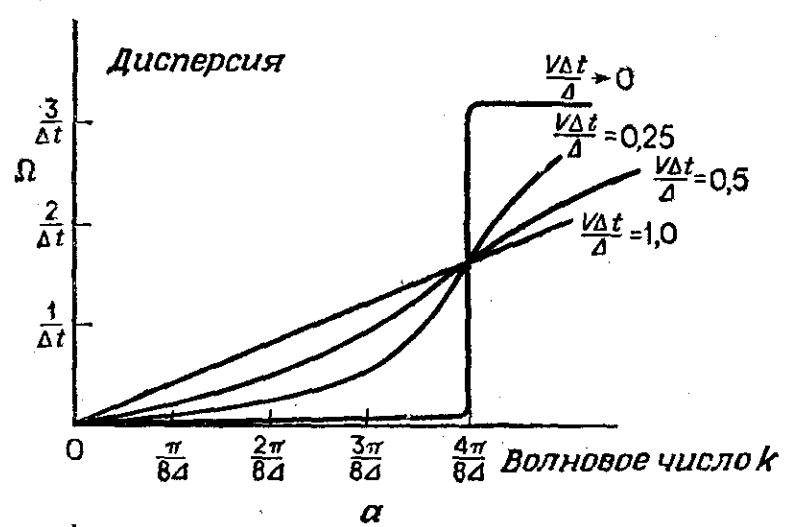
\includegraphics[width=0.45\linewidth]{figures/dispersio.png}
		\hspace{1em}
		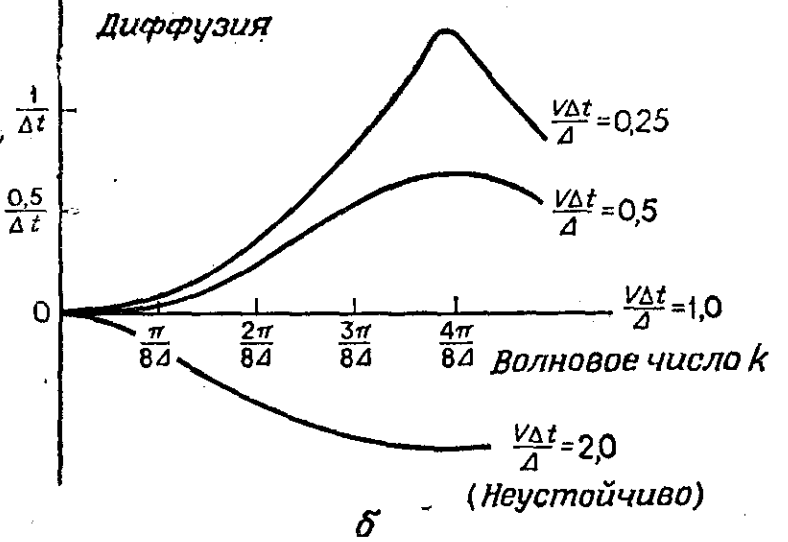
\includegraphics[width=0.39\linewidth]{figures/diffusio.png}
		\caption{а --- дисперсия, б --- диффузия в методе Лакса для уравнения переноса.}
		\label{fig:DR}
	\end{figure}
	
	\subsubsection{Порядок аппроксимации}
	Исследуем порядок аппроксимации разностной схемы Лакса для уравнения переноса. Запишем их в виде: % а кого их?
	% разностную схему Лакса и  уравнение переноса
	%А как по другому написать?
	
	\begin{align}
		& Au = 0, \\
		& A_h u_h = 0, \, \text{где} \\
		& A \equiv \frac{\partial}{\partial t} + a\frac{\partial}{\partial x}, \\
		& A_h u_h \equiv \frac{1}{2 \Delta t}\left(u_{j+1}^n -2u_j^{n+1} + u_{j-1}^n\right) - \frac{a}{2\Delta x}\left(u_{j+1}^n - u_{j-1}^n\right).\label{eq_Ah_uh}
	\end{align}
	Найдем невязку схемы
	\begin{equation}\label{discrepancy}
		\delta f = (Au - A_hu_h)_j^n 
	\end{equation}
	Используем разложение величин $u_{j-1}^n, u_{j+1}^n, u_{j}^{n+1}$ в ряд Тейлора в окрестности точки $(x_j, t^n)$:
	\begin{align}
		& u_{j-1}^n = u_j^n - \Delta x\left(\frac{\partial u}{\partial x}\right)_j^n + \frac{1}{2}\Delta x^2\left(\frac{\partial^2 u}{\partial x^2}\right)_j^n + \mathcal{O}\left(\Delta x^3\right), \\
		& u_{j+1}^n = u_j^n + \Delta x\left(\frac{\partial u}{\partial x}\right)_j^n + \frac{1}{2}\Delta x^2\left(\frac{\partial^2 u}{\partial x^2}\right)_j^n + \mathcal{O}\left(\Delta x^3\right), \\
		& u_{j}^{n+1} = u_j^n + \Delta t\left(\frac{\partial u}{\partial t}\right)_j^n + \frac{1}{2}\Delta t^2\left(\frac{\partial^2 u}{\partial t^2}\right)_j^n + \mathcal{O}\left(\Delta t^3\right). 
	\end{align}
	Подставим полученное разложение в \eqref{eq_Ah_uh} и \eqref{discrepancy}:
	\begin{align}\label{loong}
		\begin{split}
			\delta f &= \left(\frac{\partial u}{\partial t}\right)_j^n + a \left(\frac{\partial u}{\partial x}\right)_j^n - \left(\frac{1}{2\Delta t}u_j^n\right. + \frac{\Delta x}{2 \Delta t}\left(\frac{\partial u}{\partial x}\right)_j^n + \frac{\Delta x^2}{4 \Delta t}\left(\frac{\partial^2 u}{\partial x^2}\right)_j^n + \frac{\mathcal{O}\left(\Delta x^3\right)}{\Delta t} -\frac{1}{\Delta t} u_j^n -\\ &- \left(\frac{\partial u}{\partial t}\right)_j^n + \frac{\Delta t}{2} \left( \frac{\partial^2 u}{\partial t^2}\right)_j^n + \mathcal{O}\left(\Delta t^2\right) + \frac{1}{2\Delta t}u_j^n - \frac{\Delta x}{2 \Delta t}\left(\frac{\partial u}{\partial x}\right)_j^n + \frac{\Delta x^2}{4 \Delta t}\left(\frac{\partial^2 u}{\partial x^2}\right)_j^n - \frac{a}{2\Delta x}u_j^n -\\ 
			&- \frac{a}{2}\left(\frac{\partial u}{\partial x}\right)_j^n - \frac{a\Delta x}{4}\left(\frac{\partial^2 u}{\partial x^2}\right)_j^n + \mathcal{O}\left(\Delta x^2\right) + \frac{a}{2\Delta x}u_j^n - \frac{a}{2}\left(\frac{\partial u}{\partial x}\right)_j^n + \left.\frac{a\Delta x}{4}\left(\frac{\partial^2 u}{\partial x^2}\right)_j^n\right) = \\
			&= 2\left(\underbrace{\left(\frac{\partial u}{\partial t}\right)_j^n + a \left(\frac{\partial u}{\partial x}\right)_j^n}_{ =\,0}\right)  - \frac{\Delta x^2}{2 \Delta t}\left(\frac{\partial^2 u}{\partial x^2}\right)_j^n + \frac{\Delta t}{2} \left( \frac{\partial^2 u}{\partial t^2}\right)_j^n + \mathcal{O}\left(\Delta x^3\right) + \mathcal{O}\left(\Delta t^2\right) =\\ &= \mathcal{O}\left(\frac{\Delta x^2}{\Delta t}\right) + \mathcal{O}(\Delta t).
		\end{split}
	\end{align}
	В четвертой строке в \eqref{loong} первые слагаемые в скобках удовлетворяют исходному уравнению, соответвтвенно равны нулю. Если $\Delta t \sim \Delta x^2$, то третье слагаемое в выражении на~предпоследней строке будет ненулевым при любых $\Delta t$ и $\Delta x$, соответствующих условию выше. Таким образом, в уравнении появится параболическое слагаемое, то есть при таком выборе шага по времени схема не аппроксимирует уравнение переноса. Если $\Delta t \sim \Delta x$, а~это требование следует из~условия устойчивости схемы Лакса \eqref{C_laks}, доказанного выше, то третье слагаемое имеет порядок аппроксимации $\Delta x$.
	
	Итак, схема Лакса имеет <<условный>> первый порядок аппроксимации по времени $t$ и координате $x$. Другими словами, ее порядок аппроксимации $\mathcal{O}(\Delta t)+\mathcal{O}(\Delta x)$ при условии $\Delta t \sim \Delta x$.
	
	\subsection{Алгоритм решения разностной задачи}
	Рассмотрим порядок действий, который поможет решить поставленную задачу.
	\begin{itemize}
		\item [1.] Инициализация расчета:
		\begin{itemize}
			\item [1.1] считывание параметров модели,
			\item [1.2] выделение памяти динамическим переменным,
			\item [1.3] инициализация пространственной сетки,
			\item [1.4] инициализация счетчика времени,
			\item [1.5] установка начальных условий.
		\end{itemize}
		\item [2.] Основной блок расчета:
		\begin{itemize}
			\item [2.1] вычисление сеточного решения на новом временном слое,
			\item [2.2] вычисление периодических граничных условий,
			\item [2.3] обновление счетчика времени.
		\end{itemize}
		\item [3.] Завершение работы:
		\begin{itemize}
			\item [3.1] сохранение результатов в файл,
			\item [3.2] освобождение выделенной памяти.
		\end{itemize}
	\end{itemize}
	
	\section{Программная реализация}
	Реализация алгоритма была выполнена на платформе Ubuntu 22.10 в среде разработки Visual Studio Code на языке программирования C++.\\
	Основные переменные, процедуры и объекты, используемые в программе:
	\begin{itemize}
		\item Переменные для хранения входных данных
		\begin{lstlisting}
			double a, x_L, x_R, C;
			int N, M;
		\end{lstlisting}
		\item Переменные для хранения шагов сетки и по времени
		\begin{lstlisting}
			double delta_x, delta_t;
		\end{lstlisting}
		\item Переменные для хранения счетчика и времени остановки
		\begin{lstlisting}
			double t, t_stop;
		\end{lstlisting}
		\item Функции для чтения данных из файла и записи результатов в файл
		\begin{lstlisting}
			bool data_input(double& advection_rate, double& a, double& b, int& N, int& M, double& Courant_number);
			bool save_results(double* x, double* t, int N, int M, double** func);
		\end{lstlisting}
		\item Функции для выделения и освобождения памяти
		\begin{lstlisting}
			double ** create_array (size_t a, size_t b);
			void free_array (double ** m);
		\end{lstlisting}
		\item Функция инициализации расчетной сетки
		\begin{lstlisting}
			int init_grid(double* x, double* t, int N, int M, double grid_step, double time_step, double a, double b);
		\end{lstlisting}
		\item Функция установки начальных условий
		\begin{lstlisting}
			int set_ic(double** func, int N, int M, double grid_step);
		\end{lstlisting}
		\item Функция для реализации консервативного метода Лакса
		\begin{lstlisting}
			int Lax(double time_counter, double t_stop, double time_step, int N, double** func, double parameter);
		\end{lstlisting}
	\end{itemize}
	Формат ввода и вывода данных:
	\begin{itemize}
		\item Входные данные считываются из файла \texttt{input.txt};
		\item Выходные данные записываются в файл с именем \texttt{results.txt}.
	\end{itemize}
	
	\section{Результаты расчетов}
	Чтобы проанализировать работу программы, были построены различные графики зависимости $u(x)$ на языке Python с использованием библиотеки matplotlib.
	
	Сначала мы исследовали как ведут себя профили решения для фиксированного числа узлов на одном временном слое ($t = 0.03$) при изменении числа Куранта. Для этого же момента времени было построено аналитическое решение $u_n$, чтобы было удобно сравнивать изменение поведения профилей. При $C > 1$ схема неустойчива и решение некорректно (на~рис.~\ref{fig:change_C} использовано значение $C = 1.1$ --- сразу наблюдаем резкие скачки, далеко выходящие за рамки теоретического решения). Уменьшение $C$ (а значит, и $\Delta t$) при~фиксированном числе узлов приводит к увеличению численной диффузии и небольшому проявлению дисперсии (см. рис.~\ref{fig:change_C}, линии для $C = 0.9$ и $C = 0.2$). Тем не менее, для~дальнейшего анализа было выбрано значение $C = 0.9$ как приемлемое.
	\begin{figure}[h]
		\centering
		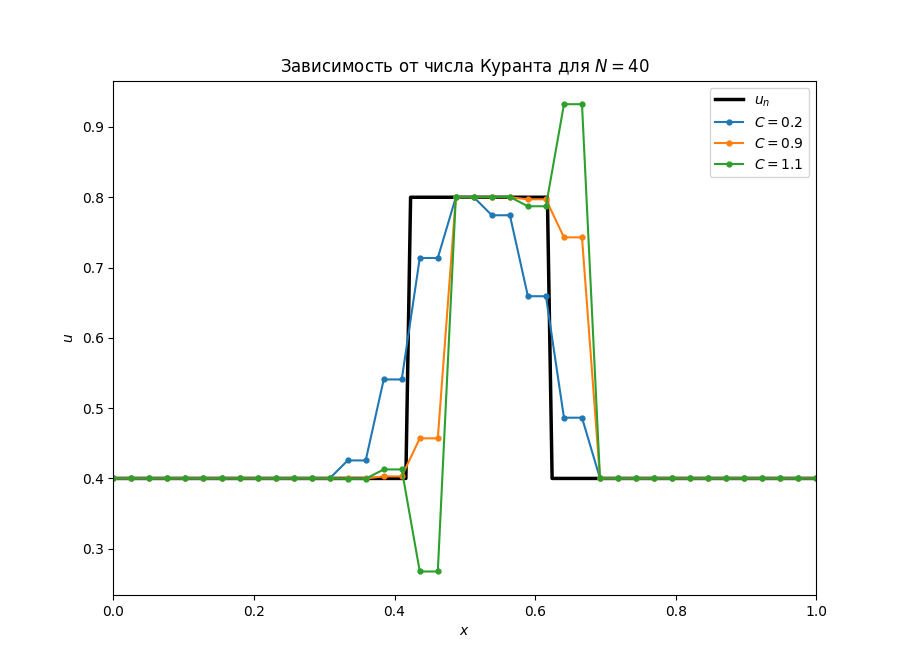
\includegraphics[width=18cm]{figures/Figure_1.png}
		\caption{Зависимость $u(x)$ от числа Куранта $C$ для числа узлов $N = 40$.}
		\label{fig:change_C}
	\end{figure}
	\begin{figure}[!h]
		\centering
		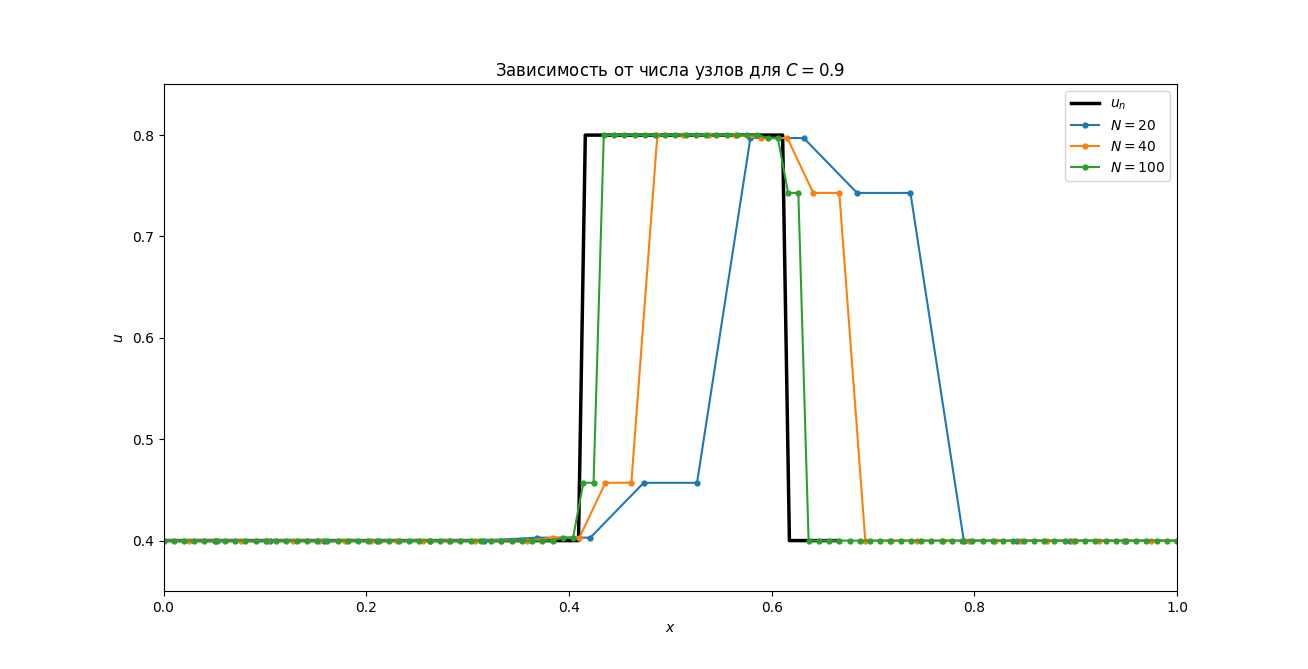
\includegraphics[width=18cm]{figures/Figure_2.png}
		\caption{Зависимость $u(x)$ от числа узлов $N$ для числа Куранта $C = 0.9$.}
		\label{fig:change_N}
	\end{figure}
	
	На рис. \ref{fig:change_N} показаны изменения профиля для заданного числа Куранта при изменяющемся числе узлов на тот же момент времени ($t = 0.03$). Сравнение с аналитическим решением $u_n$ указывает на то, что увеличение $N$ при фиксированном $C$ дает более точное решение (то есть разностное решение сходится к точному). На графике рассмотрены значения $N = 20$, $N = 40$ и $N = 100$. В первом случае мы наблюдаем сильное отклонение от теории, во втором --- это отклонение меньше, но этого недостаточно для того, чтобы свойства схемы в малой степени влияли на результат. Третий вариант, с наибольшим количеством точек, среди всех линий наилучшим образом подходит к теории, несмотря на~это мы все равно наблюдаем небольшие отклонения справа и слева от пика. Поэтому для следующего этапа выбрано значение $N = 100$, поскольку оно хорошо приближает профиль к~истинному решению.
	
	Демонстрация эволюции профиля решения уравнения переноса при выбранных параметрах приведена на рис. \ref{fig:evolution}, для~каждого момента времени было нанесено точное решение. Реализованный метод Лакса корректно описывает перенос, но приводит к заметному <<размытию>> профиля из-за численной диффузии.
	% \begin{figure}[!h]
		%     \centering
		%     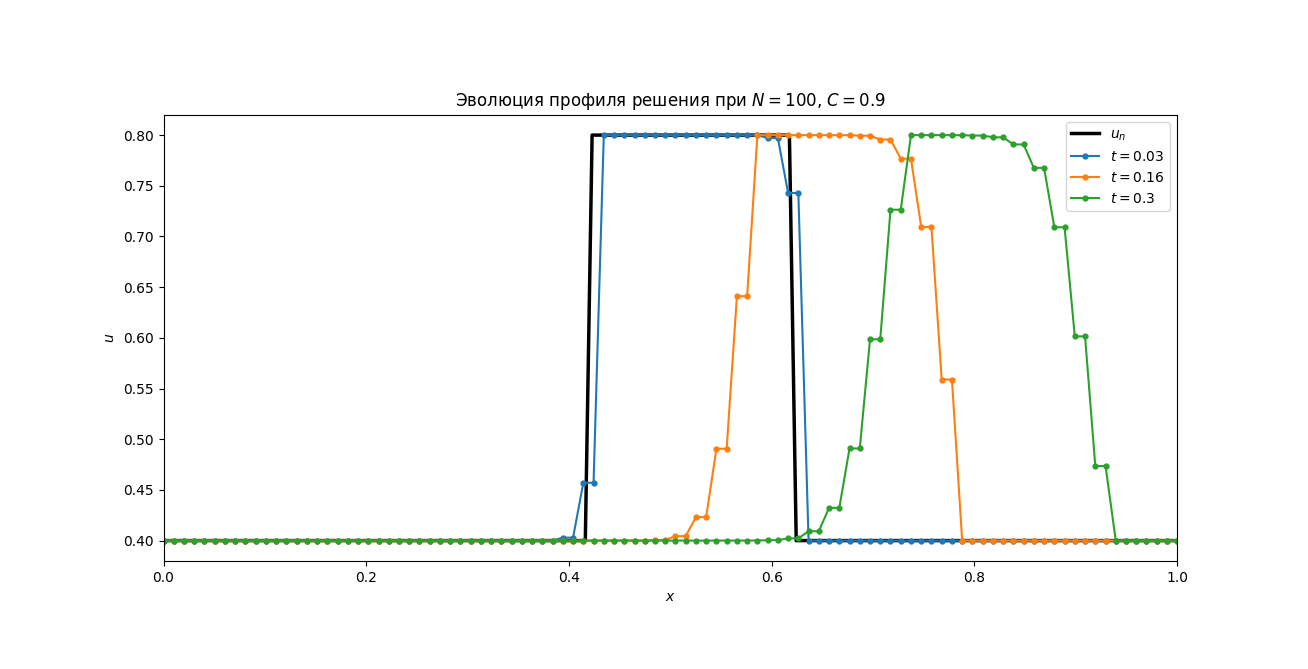
\includegraphics[width=18cm]{figures/Figure_3a.png}
		%     \caption{Эволюция профилей решения при $N=100$, $C=0.9$.}
		%     \label{fig:evolution}
		% \end{figure}
	\begin{figure}[!h]
		\centering
		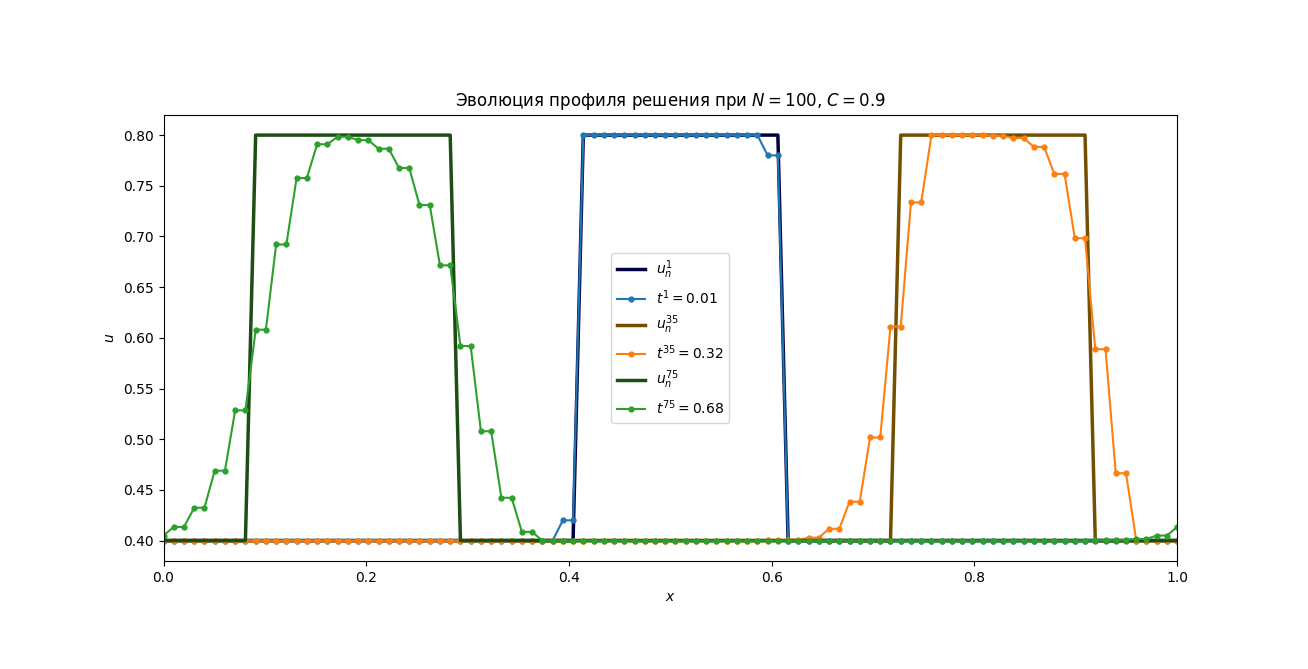
\includegraphics[width=18cm]{figures/Figure_3c.png}
		\caption{Эволюция профилей решения при $N=100$, $C=0.9$.}
		\label{fig:evolution}
	\end{figure}
	
	\section{Решение дополнительной задачи}
	\subsection{Аналитическая часть решения задачи}
	Условие задачи --- получить из системы \eqref{Maxwell1}---\eqref{Maxwell4} систему двух линейных уравнений гиперболического типа, описывающих плоскую электромагнитную волну в вакууме.
	
	Сделаем ряд упрощений, соответствующих задаче. В вакууме нет свободных электрических зарядов и проводимости, которые могли бы создавать электрический ток, следовательно, можем положить, что плотность электрического тока $\mathbf{j}$, а также объемная плотность стороннего электрического заряда $\rho$ равны нулю. Кроме того, в вакууме $\varepsilon = 1$ и $\mu = 1$ (диэлектрическая и магнитные постоянные), а~значит, справедливы соотношения (следуют из материальных уравнений)
	\begin{equation}
		\mathbf{D} = \mathbf{E}, \qquad \mathbf{B} = \mathbf{H}.
	\end{equation}
	
	На основе этих умозаключений перепишем уравнения Максвелла следующим образом
	\begin{align}
		&\nabla \cdot \mathbf{E} = 0,\label{Maxw1}\\
		&\nabla \cdot \mathbf{H} = 0,\\
		&\nabla \times \mathbf{E} = -\frac{1}{c}\frac{\partial\mathbf{H}}{\partial t},\\
		&\nabla \times \mathbf{H} = \frac{1}{c}\frac{\partial\mathbf{E}}{\partial t}.\label{Maxw4}\
	\end{align}
	
	Пусть плоская электромагнитная волна распространяется вдоль оси $x$, тогда векторы $\mathbf{E} = \{E_x, E_y, E_z\}$ и $\mathbf{H} = \{H_x, H_y, H_z\}$ не зависят от координат $y$ и $z$, поскольку амплитуда колебаний имеет постоянное значение для любой точки пространства. Таким образом, они зависят только от координаты $x$ и от времени $t$.
	% колебания векторов напряженностей электрического и магнитного полей ($\mathbf{E} \perp \mathbf{H}$):
	% \begin{equation}\label{vecE}
		%     \mathbf{E} = E_0 \cos{(\omega t - kx)}\hat{\mathbf{y}},
		% \end{equation}
	% \begin{equation}\label{vecH}
		%     \mathbf{H} = H_0 \cos{(\omega t - kx)}\hat{\mathbf{z}},
		% \end{equation}
	% где $E_0$ и $H_0$ --- амплитуды колебаний соответствующих векторов напряженностей, постоянные в любой точке пространства, $\omega$ --- круговая частота, $k = \omega/c$ --- волновое число, $c$ --- скорость света, $\hat{\mathbf{y}}$ и $\hat{\mathbf{z}}$ --- орты соответствующих осей.
	
	Вспомним свойства дифференциальных операторов, пусть $\mathbf{A} = \{A_x, A_y, A_z\}$ --- некоторый вектор, тогда
	\begin{equation}\label{div}
		\nabla \cdot \mathbf{A} \equiv \text{div}\mathbf{A} \equiv \frac{\partial A_x}{\partial x} + \frac{\partial A_y}{\partial y} + \frac{\partial A_z}{\partial z},
	\end{equation}
	\begin{equation}\label{rot}
		\nabla \times \mathbf{A} \equiv \text{rot}\mathbf{A} \equiv \left(\frac{\partial A_z}{\partial y} - \frac{\partial A_y}{\partial z}\right)\hat{\mathbf{x}} + \left(\frac{\partial A_x}{\partial z} - \frac{\partial A_z}{\partial x}\right)\hat{\mathbf{y}} + \left(\frac{\partial A_y}{\partial x} - \frac{\partial A_x}{\partial y}\right)\hat{\mathbf{z}},
	\end{equation}
	где $\hat{\mathbf{x}}$, $\hat{\mathbf{y}}$ и $\hat{\mathbf{z}}$ --- орты соответствующих осей.
	
	Применяя формулы \eqref{div} и \eqref{rot} к уравнениям Максвелла \eqref{Maxw1}---\eqref{Maxw4}, получаем
	\begin{equation}
		\frac{\partial E_x}{\partial x} = 0,
	\end{equation}
	\begin{equation}
		\frac{\partial H_x}{\partial x} = 0,
	\end{equation}
	\begin{equation}
		\frac{\partial E_z}{\partial x} = \frac{1}{c}\frac{\partial H_y}{\partial t}, \hspace{7em} \frac{\partial E_y}{\partial x} = -\frac{1}{c}\frac{\partial H_z}{\partial t},
	\end{equation}
	\begin{equation}
		\frac{\partial H_z}{\partial x} = -\frac{1}{c}\frac{\partial E_y}{\partial t}, \hspace{7em} \frac{\partial H_y}{\partial x} = \frac{1}{c}\frac{\partial E_z}{\partial t}.
	\end{equation}
	Таким образом, получаем систему дифференциальных уравнений в частных производных, описывающих плоско-поляризованную волну в вакууме (для простоты записи обозначим $E_y = E$ и $H_z = H$):
	\begin{align}
		\frac{\partial E}{\partial t} + c\,\frac{\partial H}{\partial x} = 0,\label{pEM_wave1}\\
		\frac{\partial H}{\partial t} + c\,\frac{\partial E}{\partial x} = 0.\label{pEM_wave2}
	\end{align}
	
	\subsection{Исследование устойчивости схемы}
	Исследуем решение этой системы с помощью консервативной схемы Лакса. Введем $u = \{E, H\}$ и $F = \{cH, cE\}$, тогда система \eqref{pEM_wave1}---\eqref{pEM_wave2} может быть записана в виде
	\begin{equation}\label{eq_wave}
		\frac{\partial u}{\partial t} + \frac{\partial F}{\partial x} = 0.
	\end{equation}
	Разностная схема в этом случае:
	\begin{equation}\label{dif_scheme_E}
		E_j^{n+1} = \frac{1}{2}\left(E_{j+1}^n + E_{j-1}^n\right) - \frac{c\Delta t}{2\Delta x}\left(H_{j+1}^n - H_{j-1}^n\right),
	\end{equation}
	\begin{equation}\label{dif_scheme_H}
		H_j^{n+1} = \frac{1}{2}\left(H_{j+1}^n + H_{j-1}^n\right) - \frac{c\Delta t}{2\Delta x}\left(E_{j+1}^n - E_{j-1}^n\right).
	\end{equation}
	
	Немного скажем об устойчивости такой схемы. В выражения \eqref{dif_scheme_E}---\eqref{dif_scheme_H} подставим векторную фурье-моду
	\begin{equation}
		\vec{u}^n = \left\{\widetilde{E}^n e^{ikx}, \widetilde{H}^n e^{ikx}\right\}
	\end{equation}
	и получим матрицу перехода
	\begin{equation}
		\hat{G} = 
		\begin{bmatrix}
			\cos{(k\Delta x)} & -i\,\frac{c\Delta t}{\Delta x}\sin{(k\Delta x)}\\
			-i\,\frac{c\Delta t}{\Delta x}\sin{(k\Delta x)} & \cos{(k\Delta x)}
		\end{bmatrix}.
	\end{equation}
	Найдем собственные значения $g$ матрицы $\hat{G}$
	\begin{equation}
		\left(\cos{(k\Delta x)} - g\right)^2 + \frac{c^2(\Delta t)^2}{(\Delta x)^2}\sin^2{(k\Delta x)} = 0,
	\end{equation}
	отсюда
	\begin{equation}
		g_{1,2} = \cos{(k\Delta x)} \pm \frac{ic\Delta t}{\Delta x}\sin{(k\Delta x)}.
	\end{equation}
	Полученные собственные значения относятся к волнам, распространяющимся в положительном и отрицательном направлениях вдоль оси $x$. Тем не менее, их модули совпадают:
	\begin{equation}
		|g|^2 = \cos^2{(k\Delta x)} + \frac{c^2(\Delta t)^2}{(\Delta x)^2}\sin^2{(k\Delta x)} = 1 - \sin^2{(k\Delta x)}\left(1 - \frac{c^2(\Delta t)^2}{(\Delta x)^2}\right).
	\end{equation}
	Таким образом, условие устойчивости для обеих волн:
	\begin{equation}
		\Delta t \leq \frac{\Delta x}{c}.
	\end{equation}
	В данном случае скорость света $c$ --- фазовая скорость, а не скорость переноса, но поскольку она является наибольшей на сетке, условие устойчивости совпадает с условием для уравнения переноса.
	
	Это значит, что для уравнения \eqref{eq_wave} можем применить реализованную в данной работе схему Лакса.
	
	\subsection{Численное исследование}
	Чтобы приступить к анализу решения системы \eqref{pEM_wave1}---\eqref{pEM_wave2}, выполним процедуру обезразмеривания. Пусть выполняется следующее:
	\begin{equation}\label{dimless}
		\begin{cases}
			E = e E_0, \\
			H = h E_0, \\
			t = \tau t_0, \\
			x = \widetilde{x} x_0,
		\end{cases}
	\end{equation}
	где $E_0$ (амплитуда), $t_0$ и $x_0$ являются некоторыми характерными масштабами.
	
	С помощью выражений \eqref{dimless} перепишем систему уравнений \eqref{pEM_wave1}---\eqref{pEM_wave2}:
	\begin{align}
		\frac{E_0}{t_0}\frac{\partial e}{\partial \tau} + c\,\frac{E_0}{x_0}\frac{\partial h}{\partial \widetilde{x}} = 0,\\
		\frac{E_0}{t_0}\frac{\partial h}{\partial \tau} + c\,\frac{E_0}{x_0}\frac{\partial e}{\partial \widetilde{x}} = 0.
	\end{align}
	Очевидно, что амплитуда $E_0$ в обоих уравнениях сократится, домножим каждое из них на $t_0$ и положим $t_0 = x_0 / c$, тогда
	\begin{align}
		\frac{\partial e}{\partial \tau} + \frac{\partial h}{\partial \widetilde{x}} = 0,\\
		\frac{\partial h}{\partial \tau} + \frac{\partial e}{\partial \widetilde{x}} = 0.
	\end{align}
	Теперь можем исследовать полученную систему с помощью реализованной программы, используя схему \eqref{dif_scheme_E}---\eqref{dif_scheme_H}.
	
	Зададим начальные условия, поскольку их выбор оставлен на наше умотрение, будем рассматривать распространение синусоидальных колебаний. В соответствии с характером задачи полагаем, что для нулевого момента времени справедливы следующие выражения:
	\begin{equation}
		\begin{cases}
			e(\widetilde{x},0) = \cos{(\varphi + \varphi_{e,0})},\\
			h(\widetilde{x},0) = \cos{(\varphi + \varphi_{h,0})},
		\end{cases}
	\end{equation}
	где $\varphi = 2\pi \widetilde{x} / \lambda$. Поскольку ранее провели обезразмеривание всех величин, в качестве длины волны возьмем параметр $\lambda = x_0 / 10$ (оптимальное значения для исследования данной задачи), $\varphi_{e,0}$, $\varphi_{h,0}$ --- начальные фазы компонент волны $e$ и $h$ соответственно (для простоты берем их равными нулю).
	
	\subsubsection{Результаты}
	Построение графиков производилось с помощью языка Python, для более удобного рассмотрения решения системы использовалась как 3D визуализация, так и обычная. Аналитическое решение было рассчитано из начальных условий с учетом поведения уравнения переноса, то~есть сдвигом по оси абсцисс с заданной скоростью (поскольку доступными нам методами на~данный момент обучения такое уравнение не решается чисто аналитически).
	
	Приведем несколько таких графиков для четырех моментов времени. Рассмотрим полученное решение и эволюцию каждой составляющей волны. На рис. \ref{fig:t_00} приведено решение в начальный момент времени, можно увидеть как полученные синусоиды очень хорошо приближаются к теоретическому решению.
	\begin{figure}[!h]
		\centering
		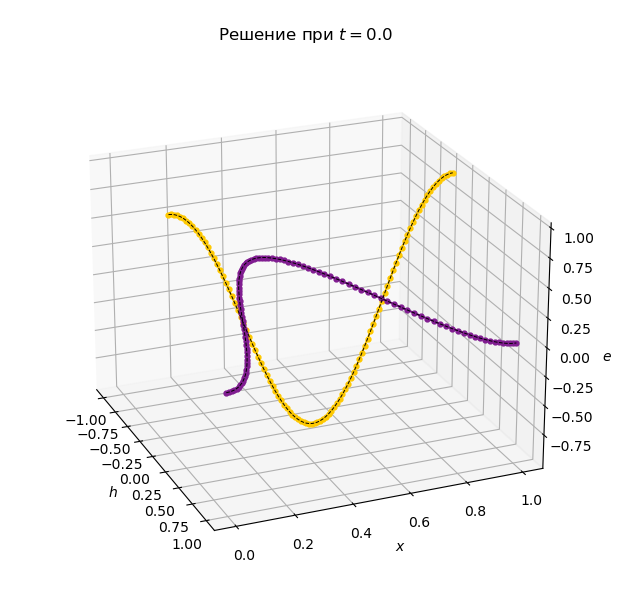
\includegraphics[width=0.45\linewidth]{figures/addd/Figure_1_t00_eh.png}
		\hspace{1em}
		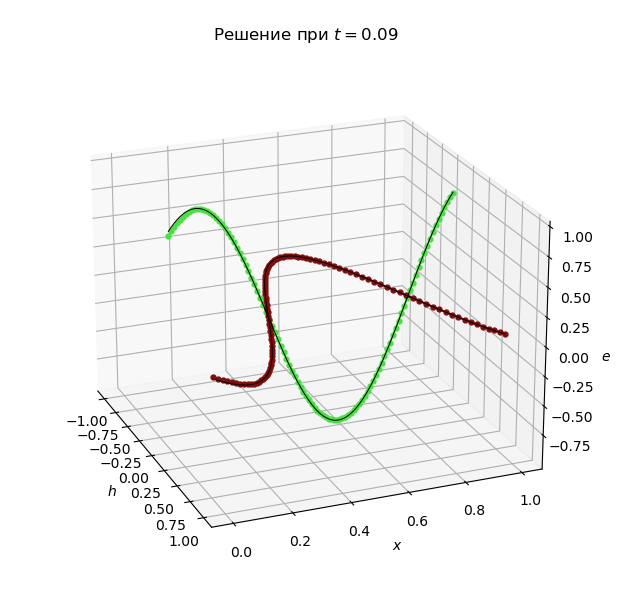
\includegraphics[width=0.45\linewidth]{figures/addd/Figure_2_t09_eh.png}
	\end{figure}
	\begin{figure}[!h]
		\centering
		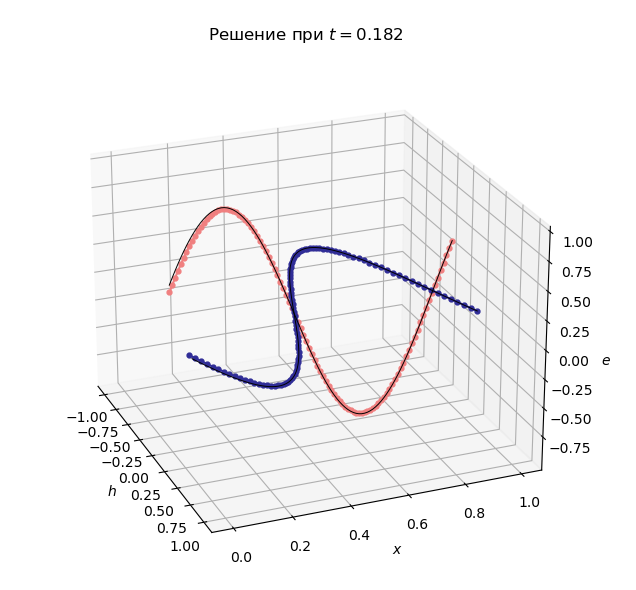
\includegraphics[width=0.45\linewidth]{figures/addd/Figure_3_t018_eh.png}
		\hspace{1em}
		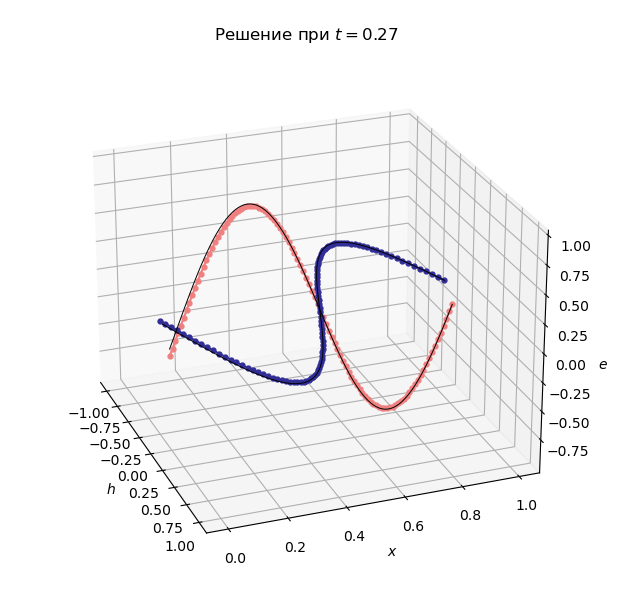
\includegraphics[width=0.45\linewidth]{figures/addd/Figure_4_t027_eh.png}
		\caption{Решение --- функции $e(x)$ и $h(x)$, описывающие движение плоской электромагнитной волны в моменты $t = 0$, $t = 0.09$, $t = 0.18$, $t = 0.27$ с нанесенными аналитическими решениями в соответствующий момент.}
		\label{fig:t_00}
	\end{figure}
	% Для~большей наглядности рассмотрим каждый профиль отдельно (см. рис. \ref{fig:t_00_z}).
	% \begin{figure}[!h]
		%     \centering
		%     \includegraphics[width=0.44\linewidth]{figures/maxwell/2d/e00sol.png}
		%     \hspace{1em}
		%     \includegraphics[width=0.44\linewidth]{figures/maxwell/2d/h00sol.png}
		%     \caption{Одномерные профили $e(x)$ и $h(x)$ в момент $t = 0$.}
		%     \label{fig:t_00_z}
		% \end{figure}
	
	% Рассмотрим решение в момент $t = 0.07$ (рис. \ref{fig:t_07}). В данном случае мы видим уменьшение амплитуды по сравнению с предыдущим моментом. Кроме того, на данном этапе решение (в особенности это видно для функции $h(x)$) начинает проявлять поведение, отклоняющееся от синусоидального. Демонстрация одномерных профилей для лушего рассмотрения представлена на рис. \ref{fig:t_07_z}.
	% \begin{figure}[!h]
		%     \centering
		%     \includegraphics[width=0.44\linewidth]{figures/maxwell/Figure_2_t07_eh.png}
		%     \hspace{1em}
		%     \includegraphics[width=0.44\linewidth]{figures/maxwell/Figure_2_t07_eh+sol.png}
		%     \caption{Решение --- функции $e(x)$ и $h(x)$, описывающие движение плоской электромагнитной волны в момент $t = 0.07$, справа добавлены аналитические функции в момент $t = 0$.}
		%     \label{fig:t_07}
		% \end{figure}
	% \begin{figure}[!h]
		%     \centering
		%     \includegraphics[width=0.44\linewidth]{figures/maxwell/2d/e07sol07.png}
		%     \hspace{1em}
		%     \includegraphics[width=0.44\linewidth]{figures/maxwell/2d/h07sol07a.png}
		%     \caption{Одномерные профили $e(x)$ и $h(x)$ в момент $t = 0.07$.}
		%     \label{fig:t_07_z}
		% \end{figure}
	
	% Аналогично в момент $t = 0.22$ (рис. \ref{fig:t_22}, \ref{fig:t_22_z}) наблюдаем еще большее уменьшение амплитуды и ее заметные скачки уже для обеих компонент. 
	% \begin{figure}[!h]
		%     \centering
		%     \includegraphics[width=0.44\linewidth]{figures/maxwell/Figure_3_t22_eh.png}
		%     \hspace{1em}
		%     \includegraphics[width=0.44\linewidth]{figures/maxwell/Figure_3_t22_eh+sol.png}
		%     \caption{Решение --- функции $e(x)$ и $h(x)$, описывающие движение плоской электромагнитной волны в момент $t = 0.22$, справа добавлены аналитические функции в момент $t = 0$.}
		%     \label{fig:t_22}
		% \end{figure}
	% \begin{figure}[!h]
		%     \centering
		%     \includegraphics[width=0.44\linewidth]{figures/maxwell/2d/e22sol22a.png}
		%     \hspace{1em}
		%     \includegraphics[width=0.44\linewidth]{figures/maxwell/2d/h22sol22.png}
		%     \caption{Одномерные профили $e(x)$ и $h(x)$ в момент $t = 0.22$.}
		%     \label{fig:t_22_z}
		% \end{figure}
	
	Эволюция для четырех моментов времени сразу представлена на рис. \ref{fig:eh_evol}. Для обеих составляющих были заданы одинаковые начальные условия, следовательно, эволюция выглядит одинаково. На этих графиках можно заметить небольшие отклонения на краях промежутка от аналитического решения.
	\begin{figure}[!h]
		\centering
		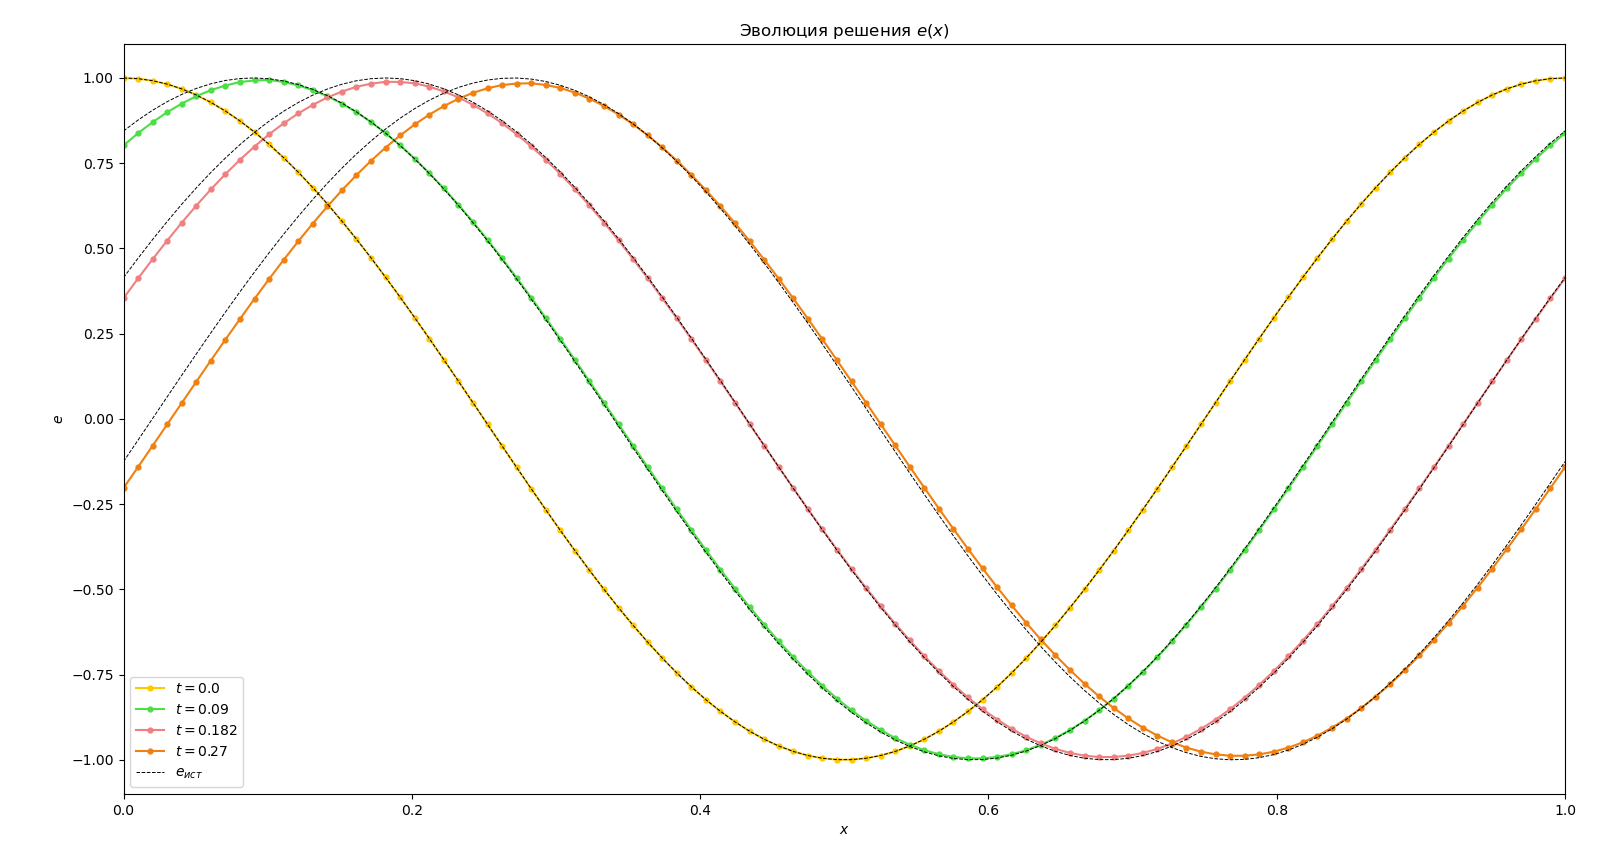
\includegraphics[width=17cm\linewidth]{figures/addd/evol_e.png}
	\end{figure}
	\begin{figure}[!h]
		\centering
		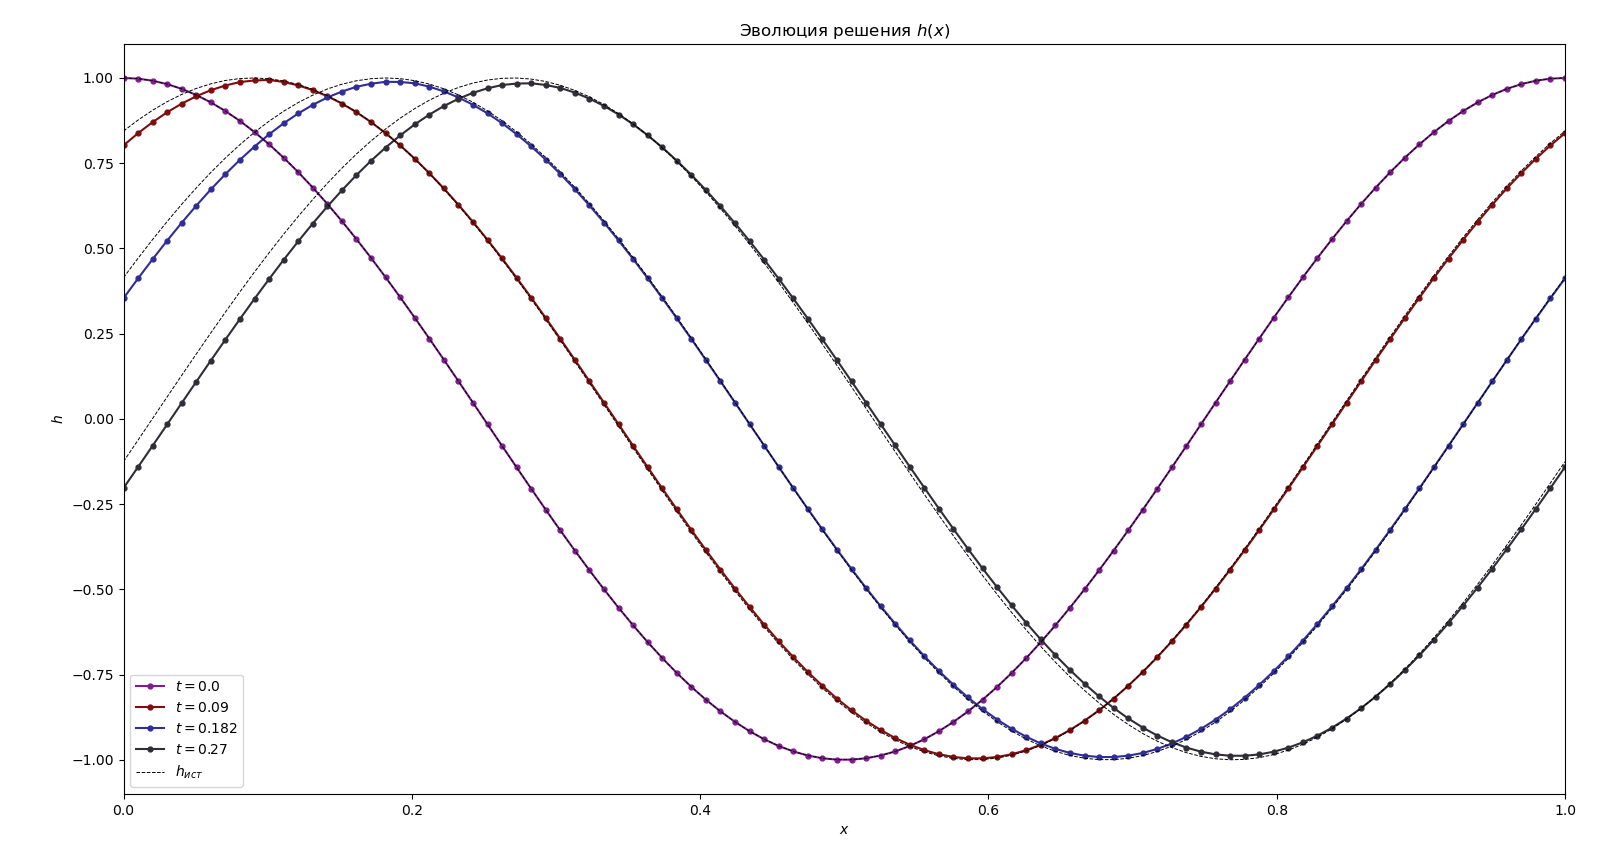
\includegraphics[width=17cm\linewidth]{figures/addd/evol_h.png}
		\caption{Эволюция одномерных профилей $e(x)$ и $h(x)$.}
		\label{fig:eh_evol}
	\end{figure}
	
	
	% Исследуемая волна затухает и перестает вести себя как синусоида. В вакууме такое поведение для электромагнитной волны невозможно. Можно сделать предположение, что в данном явлении наибольший вклад вносит схема Лакса, которая имеет первый порядок аппроксимации и заметно ухудшает решение с течением времени.
	
	\newpage
	\section{Заключение}
	В данной работе был исследован консервативный метод Лакса для численного решения одномерного уравнения переноса. Были проведены аналитические исследования устойчивости, диффузии и дисперсии на сетке, а также порядка аппроксимации разностной схемы Лакса. Была разработана и реализована программа для ЭВМ, которая позволяет решать указанные задачи с использованием метода Лакса.
	
	Анализ результатов показал, что реализованный метод Лакса корректно описывает перенос, но приводит к заметному размытию профиля из-за численной диффузии. Точность решения можно улучшить путем увеличения числа узлов сетки.
	
	Была решена дополнительная задача, из уравнений Максвелла была получена система линейных уравнений гиперболического типа. Исследование численного решения этой системы привело к получению графиков, которые описывают поведение плоской электромагнитной волны в вакууме. Данная схема, несмотря на ее свойства, ограничивающие возможность получения точного решения, вполне корректно описывает решение поставленной задачи: мы видим лишь небольшие отклонения в поведении электрической и магнитной компонент волны.
	
	Данная работа является важным шагом в изучении численных методов для решения уравнений переноса и гиперболических уравнений в целом, а также может быть использована в качестве основы для дальнейших исследований в этой области.
	
	% \newpage
	\begin{thebibliography}{4}
		\bibitem{book_optics} Литвинов О.С., Горелик В.С. Электромагнитные волны и оптика: учеб. пособие для~вузов --- М.: Изд-во МГТУ им. Н.Э. Баумана, 2006. --- 446 с.
		
		\bibitem{book_nummeth} Randall J. LeVeque Numerical methods for conservation laws --- Birkhäuser Verlag, Basel, 1992. --- 214 p.
		
		\bibitem{book_numphys} Поттер Д. Вычислительные методы в физике --- М.: Мир, 1975. --- 392 с.
		
		% ПРИМЕРЫ:
		% \bibitem{article} Гуреев В.Н., Мазов Н.А. Использование библиометрии для оценки значимости журналов в научных библиотеках (обзор) // Научно-техническая информация. Сер. 1. --- 2015. --- № 2. --- С. 8—19.
		
		% \bibitem{url} Web of Science. --- URL: http://apps.webofknowledge.com/ (дата обращения 15.11.2016).
	\end{thebibliography}
	
\end{document}
